\subsubsection{Volume e encadeamento das simulações}
\noindent Com a confirmação do número de parâmetros e variáveis necessários para a etapa de simulação, foi analisada a quantidade de interações entre as variáveis definidas. Esta análise visou apontar a viabilidade de execução do volume de simulação para a determinação da eficiência energética dos modelos com o aparato computacional disponível.\vspace*{0.3cm} \newline
\noindent Para tal, utilizou-se uma análise combinatória simples, onde foram combinados entre si os números de 9 parâmetros e 24 variáveis, como apresentado na Tabela \ref{tab:tabela9}. O resultado da análise, sem importância de ordem entre os elementos e sem repetição de ordem entre as variáveis, foi de 1.307.504 possibilidades de combinação. Considerando que a capacidade computacional disponível para a análise de todas essas possibilidades é limitada e que o tempo de simulação para cada possibilidade, neste trabalho tratada como cenário, é curto \cite{Werneck2017}, porém, dado o volume de cenários, torna-se impraticável dentro do tempo de desenvolvimento estipulado para a conclusão do trabalho.\vspace*{0.3cm} \newline
\noindent Dada a quantidade de combinações, optou-se pela fixação de 6 parâmetros, ou seja, sistemas de condicionamento de ar; medidas de redução de carga de energia de iluminação e equipamentos; transmitâncias de paredes, cobertura e proteção solar; e alteração de 3 parâmetros, de forma sequencial, sendo eles o PAF\textsubscript{T}; vidro; e a orientação solar, criando, assim, 192 cenários para cada modelo genérico, totalizando 384 cenários.\vspace*{0.3cm} \newline
\noindent A criação destes cenários tem como finalidade a redução do volume de simulações e evidenciar a influência das variáveis arquitetônicas sobre as edificações criadas. Baseado em ASHRAE et al. \citeyear{AmericanSocietyofHeatingRefrigeratingandAir-ConditioningEngineers-ASHRAE2019}, Costa \citeyear{Costa2018}, e Veloso \citeyear{Veloso2017}, os cenários foram segmentados em 10 blocos de simulação, segmentação esta apresentada pela Figura \ref{fig:figura13}. Os blocos de simulação com variáveis fixas representam as implementações incrementais de medida de redução de consumo de energia, enquanto os blocos com variáveis aleatórias são implementados em todos os cenários.\pagebreak
\begin{figure}[H]
    \centering
    \caption{Descrição simplificada dos blocos de simulação.}
    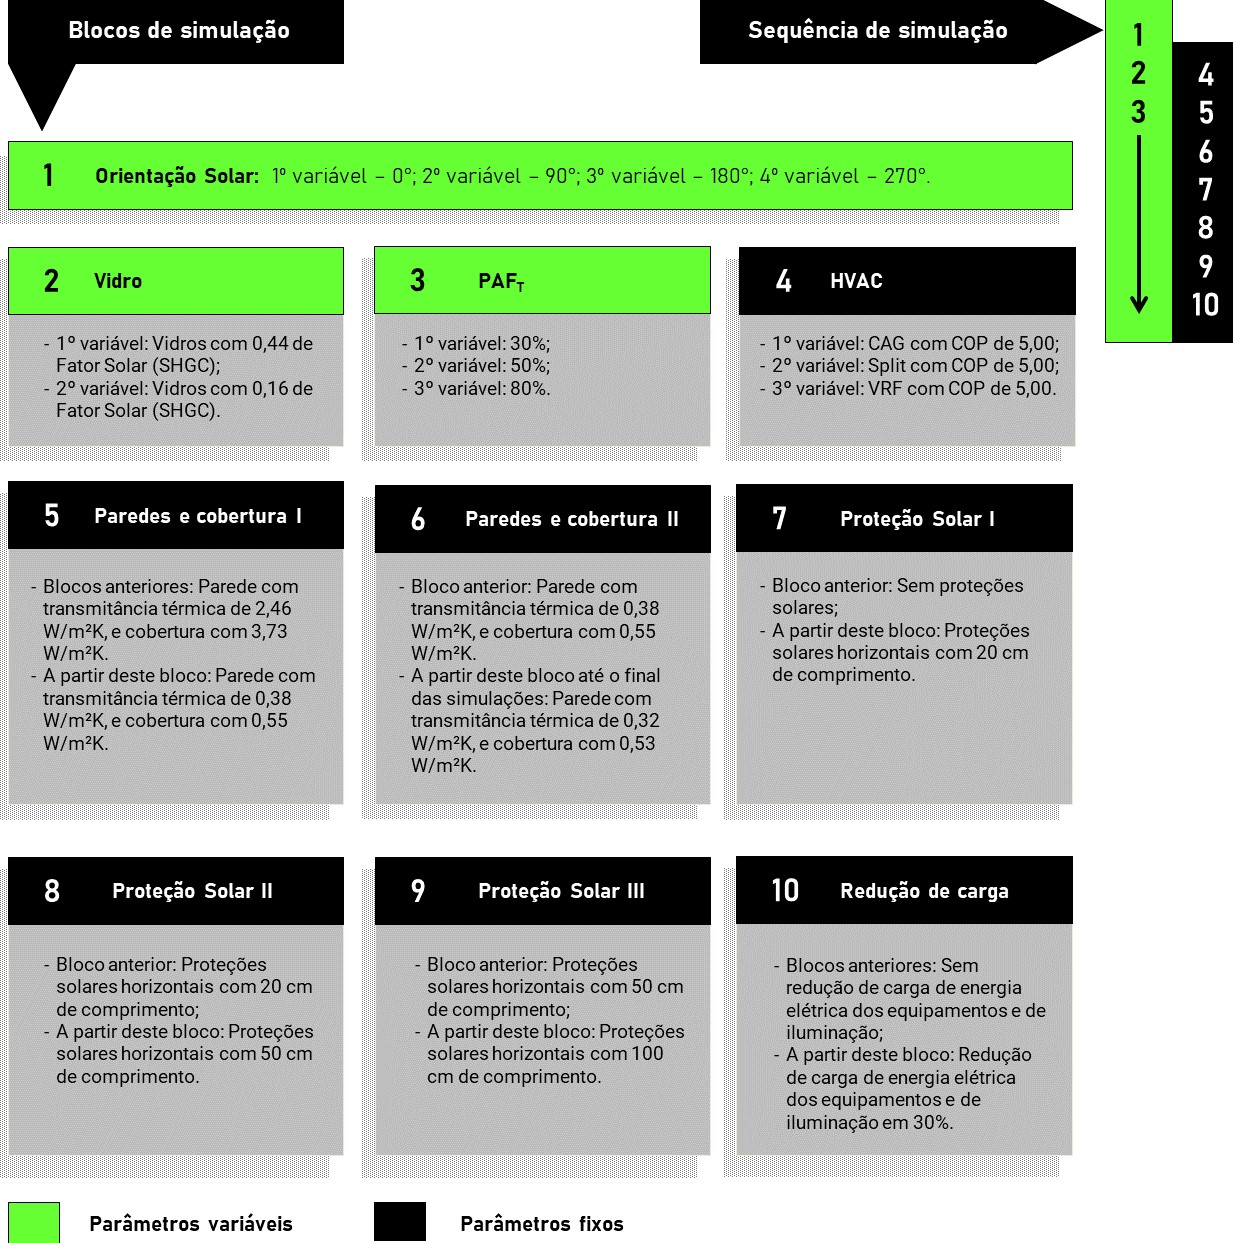
\includegraphics[width=1.0\textwidth]{figures/fig13-fluxograma.jpg}
    \begin{flushleft}
        \par \small Fonte: autor (2019)
    \end{flushleft}
    \label{fig:figura13}
\end{figure}
\noindent Tendo em vista os parâmetros apresentados na Tabela 10, os blocos de simulação são compostos por características básicas atribuídas para a envoltória, materiais e componentes, sistemas de condicionamento de ar, iluminação e equipamentos, características estas representadas pelas variáveis “a”. Da mesma forma, as implementações de redução de consumo de energia são apresentadas pelas variáveis “b”, “c” e “d”.\vspace*{0.3cm} \newline
\noindent Do primeiro ao terceiro bloco de simulações, compostos por 32 cenários, foram variadas as características de orientação solar, vidros e PAF\textsubscript{T} das edificações propostas. Concomitante à implementação do bloco de simulação 2, o sistema de condicionamento de ar “a”, sistema presente no levantamento, foi substituído pela opção “b”, sistema mais eficiente proposto. Deste ponto em diante, os blocos 4 a 10 foram implementados sequencialmente aos blocos de simulação 1 a 3. Todavia, as variáveis foram analisadas isoladamente cujas análises encontram-se relatadas no capítulo sobre o impacto das variáveis sobre o consumo anual de energia elétrica.\vspace*{0.3cm} \newline
\noindent Após os blocos 1 a 3 iniciados, foram inseridos, ao longo da sequência de simulações, os 7 blocos de simulação com variáveis fixas, compostos por 24 cenários cada. Estes blocos são compostos por sistemas de condicionamento de ar, alteração dos parâmetros de composição construtiva de paredes e cobertura, inserção de proteções solares e medidas de redução de consumo de carga de energia elétrica para equipamentos e iluminação. Estas variáveis fixas foram implementadas de forma incremental e sequencial, de acordo com a finalização da simulação precedente, a fim de evidenciar a influência de cada medida sobre o consumo energético.\vspace*{0.3cm} \newline
\noindent Com a conclusão do encadeamento de sequência das simulações, pôde-se desenvolver o processo de modelagem dedicado aos blocos de simulação.